\documentclass[14pt]{article}
\usepackage{ucs}
\usepackage[utf8x]{inputenc} % Включаем поддержку UTF8
\usepackage[russian]{babel} 
\usepackage{graphicx}
\usepackage{listings}
\usepackage{xcolor}
\lstset { %
    language=C++,
    backgroundcolor=\color{black!5}, % set backgroundcolor
    basicstyle=\footnotesize,% basic font setting
}

\begin{document}

\section{ROI}
\subsection{Описание}
Назовем глубиной пикселя минимальное число шагов (вверх, вниз, влево, вправо), необходимое, чтобы достичь пиксель другого цвета или границу изображения. 
\begin{figure}[ht]
    \centering
    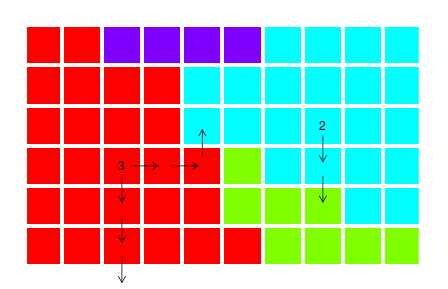
\includegraphics[width=0.75\linewidth]{pixeldepthspic.png}
    \caption{\label{fig:demo} Пиксель, помеченный как 3, имеет глубину 3, так как необходимо минимум 3 шага для того, чтобы достичь пикселя с отличным от красного цветом. Шаги не всегда выполняются в одном направлении. Аналогично, пиксель, помеченный как 2, имеет глубину 2. Зеленые и фиолетовые пиксели имеют глубину 1. }
\end{figure}

Требуется написать функцию:
\begin{lstlisting}
PixelArray max_depth_pixels(Image const* image, unsigned color);
\end{lstlisting}
которая принимает изображение в виде структуры \textbf{Image} и цвет пикселя \textbf{color}. Результатом работы функции является массив структур \textbf{Points}, который хранит индексы всех пикселей с максимальной глубиной и количество этих точек, упакованный в структуру \textbf{PixelArray}. 

Изображение задается структурой:
\begin{lstlisting}
struct Image{
  unsigned *pixels;   
  unsigned long width, height;
};
\end{lstlisting}
в виде двумерного массива, упакованного по строкам в одномерный массив. Цвет пикселя задается целым положительным числом меньшим $2^{32}$, ширина и высота изображения представлена целыми, положительными числами, 
лежащими в диапазоне $1 \le \mathrm{width, height} \le 100000$.

Вспомогательные структуры имеют вид:
\begin{lstlisting}
struct Points{
  unsigned long x; //row index
  unsigned long y; //column index
};
struct PixelArray{
  Points* pixels;
  unsigned long long size;
};
\end{lstlisting}

\textit{Примечание: учитывая большие размеры изображений, эффективный алгоритм должен иметь сложность $O(nm)$.}
\subsection{Тестирование, входные и выходные данные}
Для тестирования кода и сдачи решения использовать файл \textbf{roi.cpp}.

\section{Повторения}
\subsection{Описание}
Написать функцию
\begin{lstlisting}
    struct NumericSeq{
      long *begin = nullptr, *end = nullptr;
    };
    
    NumericSeq remove_elements(NumericSeq input, unsigned long N);
\end{lstlisting}
которая принимает последовательность чисел $-10^9 \le A_i \le 10^9$, число $2 \le N \le 9$ и удаляет из нее все элементы, которые встречаются в ней более $N$ раз, начиная с $N+1-го$ вхождения ($N$ дубликатов удаляемого элемента остается в последовательности). Порядок остальных элементов остается неизменным. 

\textit{Например:}
Дана последовательность $A = [1,2,3,1,2,1,2,3]$ и число $N~=~2$. После выполнения функции последовательность будет иметь вид $[1,2,3,1,2,3]$.

Для $[1,1,1,1]$, $N=2$ --- $[1, 1]$,

для $[20,37,20,21]$, $N=1$ --- $[20, 37, 21]$.

\subsection{Тестирование, входные и выходные данные}
Для тестирования кода и сдачи решения использовать файл \textbf{occurrences.cpp}.

\section{Smallest possible sum}
\subsection{Описание}

Дан массив целых, положительных чисел $X$, $1 \le X[i] \le 1000000$. Для каждой пары $X[i] и X[j]$ элементов массива
выполняется преобразование:
\begin{lstlisting}
if X[i] > X[j] then X[i] = X[i] - X[j]
\end{lstlisting}
Когда в массиве не остается больше пар элементов, для которых можно выполнить приведенное выше преобразования,
выполняется подсчет суммы элементов. Полученную сумму будем называть наименьшей возможной суммой (я хз откуда такое название).

\textit{Например:}
\begin{verbatim}
X_1 = [6, 9, 12] # -> X_1[2] = X[2] - X[1] = 21 - 9
X_2 = [6, 9, 6]  # -> X_2[2] = X_1[2] - X_1[0] = 12 - 6
X_3 = [6, 3, 6]  # -> X_3[1] = X_2[1] - X_2[0] = 9 - 6
X_4 = [6, 3, 3]  # -> X_4[2] = X_3[2] - X_3[1] = 6 - 3
X_5 = [3, 3, 3]  # -> X_5[1] = X_4[0] - X_4[1] = 6 - 3
\end{verbatim}
Наименьшая возможная сумма для этого массива равна 9.

Необходимо написать функцию
\begin{lstlisting}
unsigned long long lps(unsigned long long *begin, unsigned long long *end);
\end{lstlisting}
которая принимает указатели на начало и конец последовательности $X$ и возвращает наименьшую возможную сумму.

\subsection{Тестирование, входные и выходные данные}
Для тестирования кода и сдачи решения использовать файл \textbf{lsp.cpp}.
\end{document}


